% !TEX encoding = UTF-8 Unicode

\documentclass[twocolumn,10pt,a4j]{ltjsarticle}
\usepackage{kougai}

\title{ゲームに最適化されたベンチマークソフトの開発}
\author{2032087 大司 陽輝  指導教員 須田 宇宙 准教授}
\date{}

\begin{document}

\maketitle

\section{はじめに}
近年では,CPUやGPUの発展に伴いゲームの需要が増加し,その中でも,よりグラフィカルで表現力のあるゲーミングPCが注目される.しかし,ゲーミングPCを購入するには専門的な知識を要する.
ベンチマークソフトを使うことでパソコンの客観的な性能を図ることができるが,ゲームによって要求されるスペックが異なるため既存のベンチマークソフトでは不十分である.

そこで本研究では各処理装置に自由に負荷をかけられるベンチマークソフトの開発を行うことを目的とする.

\section{ゲームについて}
近年のゲームは,昔に比べリアルなグラフィックに近づけるため,草木などに物理法則に則った動きが追加や,ポリゴン数が増え解像度の高いテクスチャが使用されるようになった,図1は,サンプルとして鮮明感がわかるよう宇宙のテクスチャを用意した.左側の球体は高い解像度のテクスチャを使用し,右側は低い解像度のテクスチャを使用している.高い解像度のテクスチャを使用することではっきりとした絵になり,リアルなグラフィックになるが,GPU・VRAMに負荷が掛かりその負荷のかかり方や量はゲームによって異なる.そこで,ゲームが求める各パーツの性能に対して,性能が劣っていると,画像の描画が遅れ(フレームレートが低下し)スムーズにプレイすることができなくなる.%なったり,描画の品質を落とす必要が出てくる.

既存のベンチマークでは,ゲームごとに掛かる負荷が異なることに対して,負荷の再現度が低い.
既存のベンチマークでは,CPUのみに負荷をかけたり,GPUのみに負荷をかけたり,一つのゲームタイトルのみの参考値しか提示されなかったりと,各ゲームへの参考とするには不十分である.
%物理演算やNPCの思考ルーチンの処理を行うためにCPUの性能を重視するゲームや,影や高いテクスチャの解像度でリアルなグラフィックの処理を行うGPU・VRAMの性能を重視するゲームや,その両方を求められるゲームがある.

\begin{figure}[H]
\begin{center}
 \includegraphics[clip,width=80mm,height=25mm]{sample_01.jpg}
\end{center}
 \caption{テクスチャの解像度の違いによる見え方の違い}
 \label{fig:図1}
\end{figure}
\vspace{-2mm}


\section{実装}
本研究では,オブジェクト数とポリゴン数を変動させることで,CPUに負荷がかけられると考え,テクスチャの解像度の変更とシェーダーの変更でGPUとVRAMに負荷を掛けられることでゲームを模すことができると検討し,Unityで実装を行った様子を図2に示す.

\vspace{2mm}
\begin{figure}[H]
\begin{center}
 \includegraphics[clip,width=80mm,height=35mm]{FlexBench.png}
\end{center}
 \caption{開発を行ったソフト}
 \label{fig:図1}
\end{figure}

\section{結果}
オープンワールドのゲームではプレイヤーに,約1万7千ポリゴン,サブキャラクターに約5千ポリゴン,敵キャラクターに3千~1万2千ポリゴン使用される,テクスチャは一枚あたり数MBから数十MBになることが多い.そこで本研究では,上記の情報をもとにし,さらにステージのポリゴン数1万ポリゴン,草や木などのオブジェクトを数個~数十個の1オブジェクトあたり500ポリゴン,シェーダーはStandardと仮設とし,様々な性能のハードウェアで検証を行った結果を図2と,表1の対応表にて示す.図2の数値は,ベンチマークソフト実行時のフレームレートの違いを示しており,数値が高いほど,性能に余裕があり,快適であることが示される.結果から,ゲームのポリゴン数や,テクスチャ容量を模した上で各構成にてフレームレートの違いを計測することができた.

\vspace{5mm}
\begin{figure}[H]
\begin{center}
 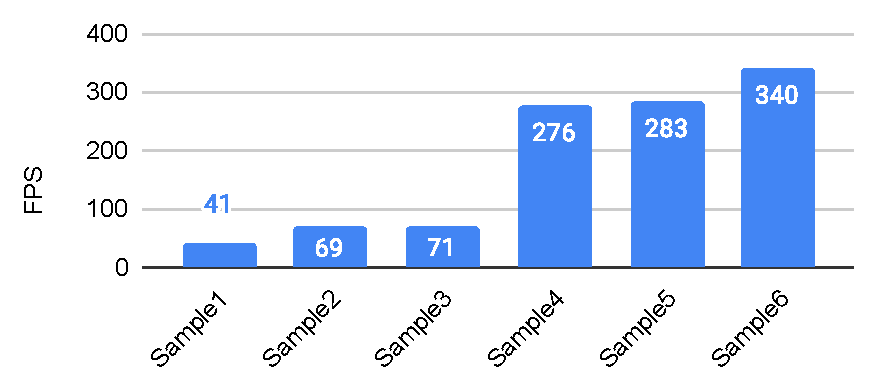
\includegraphics[clip,width=70mm,height=35mm]{グラフ.pdf}
\end{center}
 \caption{各厚生でのフレームレート}
 \label{fig:図1}
\end{figure}

\vspace{5mm}
\begin{table}[H]
\begin{center}
\caption{ハードウェア構成の対応表}
\vspace{2mm}
 \label{fig:教科書}
 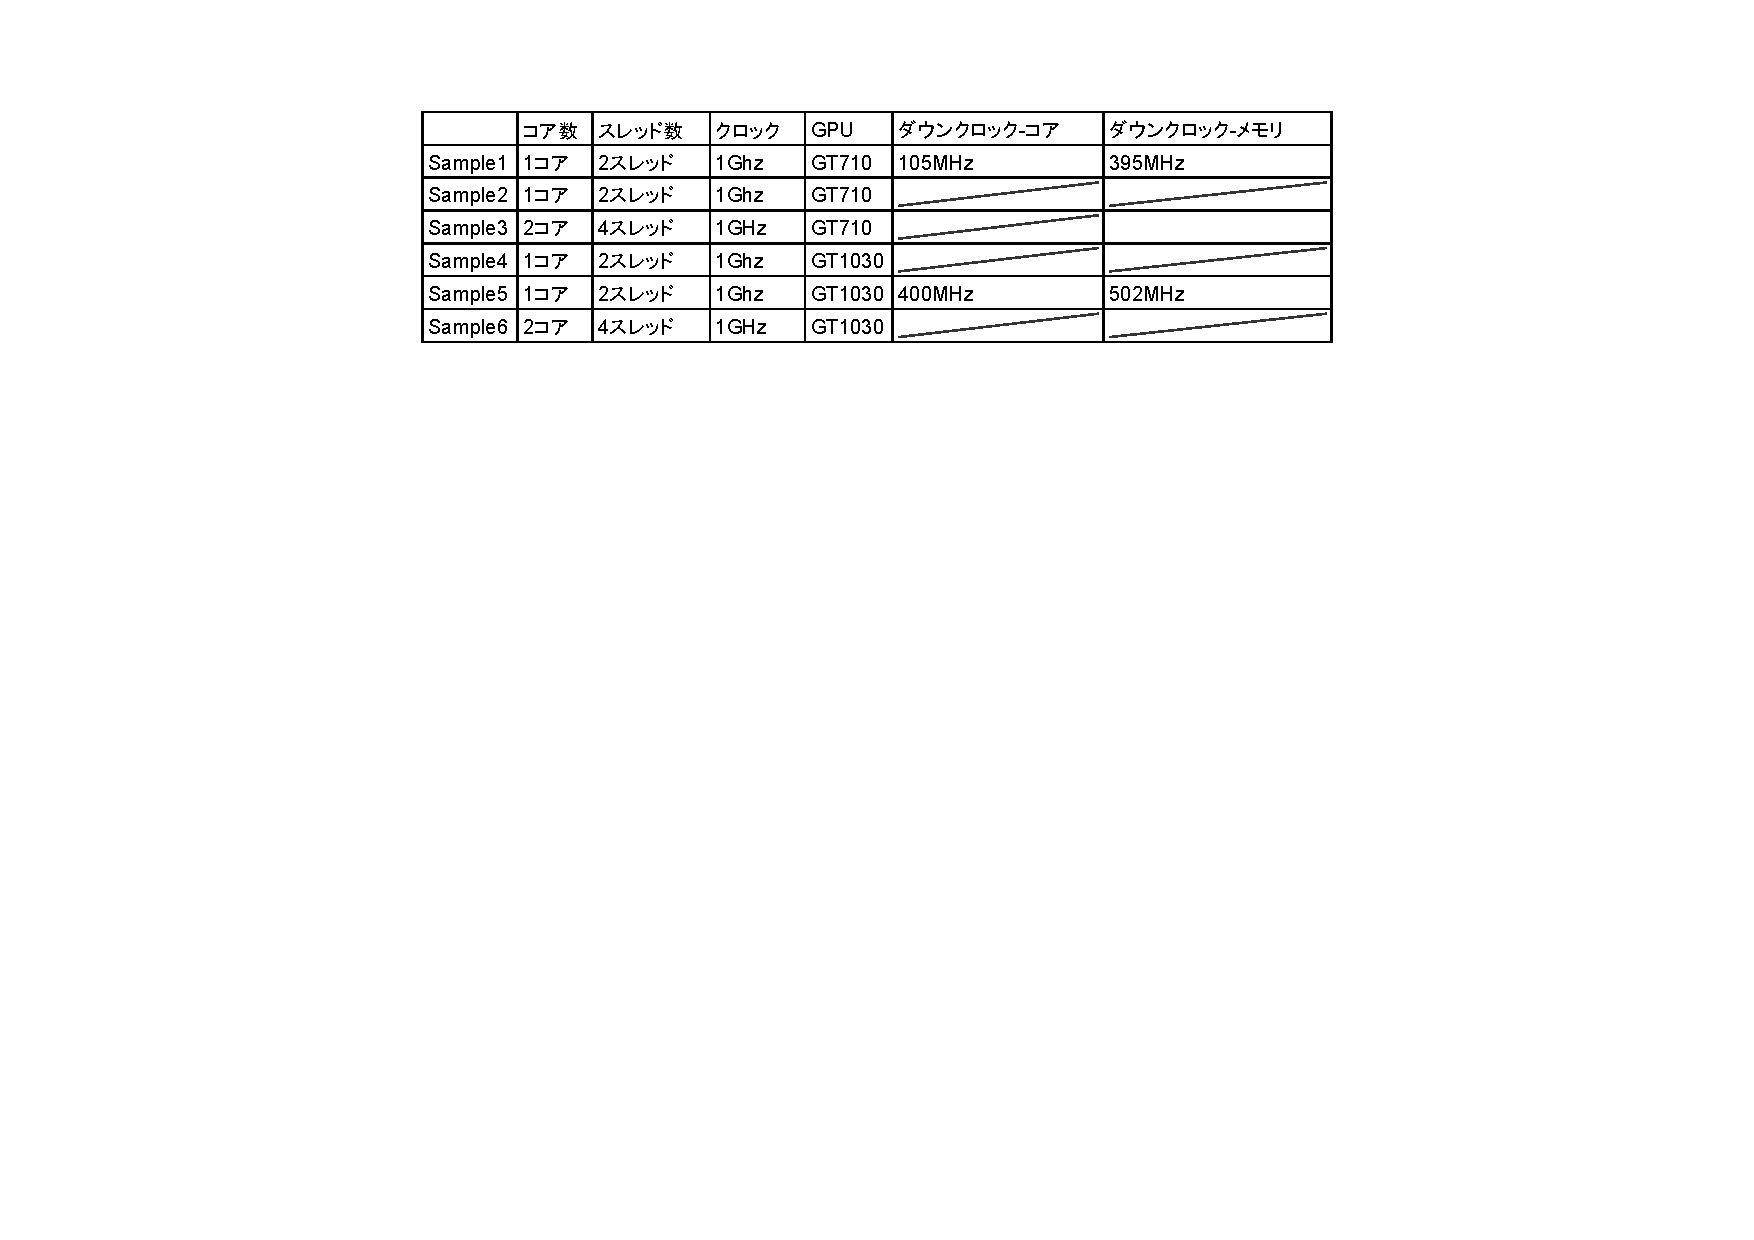
\includegraphics[clip,width=65mm,height=25mm]{対応表.pdf}
\end{center}
\end{table}

\vspace{-2mm}
\section{終わりに}
\vspace{-1mm}
本研究では,ポリゴン数やオブジェクト数を変更できるソフトを開発することで,ゲームの処理を模し,ゲームの負荷を再現することができ不足しているパーツの性能を明確にすることができた.今後は,機能を追加することでさらに忠実にしていきたい.


\end{document}
